%%%%%%%%%%%%%%%%%%%%%%%%%%%%%%%%%%%%%%%%%
% Beamer Presentation
% LaTeX Template
% Version 1.0 (10/11/12)
%
% This template has been downloaded from:
% http://www.LaTeXTemplates.com
%
% License:
% CC BY-NC-SA 3.0 (http://creativecommons.org/licenses/by-nc-sa/3.0/)
%
%%%%%%%%%%%%%%%%%%%%%%%%%%%%%%%%%%%%%%%%%

%----------------------------------------------------------------------------------------
%	PACKAGES AND THEMES
%----------------------------------------------------------------------------------------

\documentclass{beamer}

\mode<presentation> {

% The Beamer class comes with a number of default slide themes
% which change the colors and layouts of slides. Below this is a list
% of all the themes, uncomment each in turn to see what they look like.

%\usetheme{default}
%\usetheme{AnnArbor}
%\usetheme{Antibes}
%\usetheme{Bergen}
%\usetheme{Berkeley}
%\usetheme{Berlin}
%\usetheme{Boadilla}
%\usetheme{CambridgeUS}
%\usetheme{Copenhagen}
%\usetheme{Darmstadt}
%\usetheme{Dresden}
%\usetheme{Frankfurt}
%\usetheme{Goettingen}
%\usetheme{Hannover}
%\usetheme{Ilmenau}
%\usetheme{JuanLesPins}
%\usetheme{Luebeck}
\usetheme{Madrid}
%\usetheme{Malmoe}
%\usetheme{Marburg}
%\usetheme{Montpellier}
%\usetheme{PaloAlto}
%\usetheme{Pittsburgh}
%\usetheme{Rochester}
%\usetheme{Singapore}
%\usetheme{Szeged}
%\usetheme{Warsaw}

% As well as themes, the Beamer class has a number of color themes
% for any slide theme. Uncomment each of these in turn to see how it
% changes the colors of your current slide theme.

%\usecolortheme{albatross}
%\usecolortheme{beaver}
%\usecolortheme{beetle}
%\usecolortheme{crane}
%\usecolortheme{dolphin}
%\usecolortheme{dove}
%\usecolortheme{fly}
%\usecolortheme{lily}
%\usecolortheme{orchid}
%\usecolortheme{rose}
%\usecolortheme{seagull}
%\usecolortheme{seahorse}
%\usecolortheme{whale}
%\usecolortheme{wolverine}

%\setbeamertemplate{footline} % To remove the footer line in all slides uncomment this line
%\setbeamertemplate{footline}[page number] % To replace the footer line in all slides with a simple slide count uncomment this line

%\setbeamertemplate{navigation symbols}{} % To remove the navigation symbols from the bottom of all slides uncomment this line
}

\usepackage{graphicx} % Allows including images
\usepackage{booktabs} % Allows the use of \toprule, \midrule and \bottomrule in tables

\usepackage[utf8]{inputenc}% A modifier en fonction du codage d'entrée
\usepackage[T1]{fontenc}
\usepackage{lmodern}% Ou autre fonte

 \usepackage[french]{babel}
%----------------------------------------------------------------------------------------
%	TITLE PAGE
%----------------------------------------------------------------------------------------

\title[Démineur]{Développement Mobile - Démineur} % The short title appears at the bottom of every slide, the full title is only on the title page

\author{Kamarouzamane Combo et Jérémy Legros} % Your name

\date{\today} % Date, can be changed to a custom date

\begin{document}

\begin{frame}
\titlepage % Print the title page as the first slide
\end{frame}

\begin{frame}
\frametitle{Sommaire} % Table of contents slide, comment this block out to remove it
\tableofcontents % Throughout your presentation, if you choose to use \section{} and \subsection{} commands, these will automatically be printed on this slide as an overview of your presentation
\end{frame}

%----------------------------------------------------------------------------------------
%	PRESENTATION SLIDES
%----------------------------------------------------------------------------------------

%------------------------------------------------
\section{Introduction}
%------------------------------------------------

%\subsection{Subsection Example} % A subsection can be created just before a set of slides with a common theme to further break down your presentation into chunks


\begin{frame}
	\frametitle{Conception UML}
	\begin{block}{Définition}
 		UML : Unified modeling language
	\end{block}
\end{frame}


\begin{frame}
	\frametitle{Conception UML}
	\begin{block}{Diagramme de classe}
 		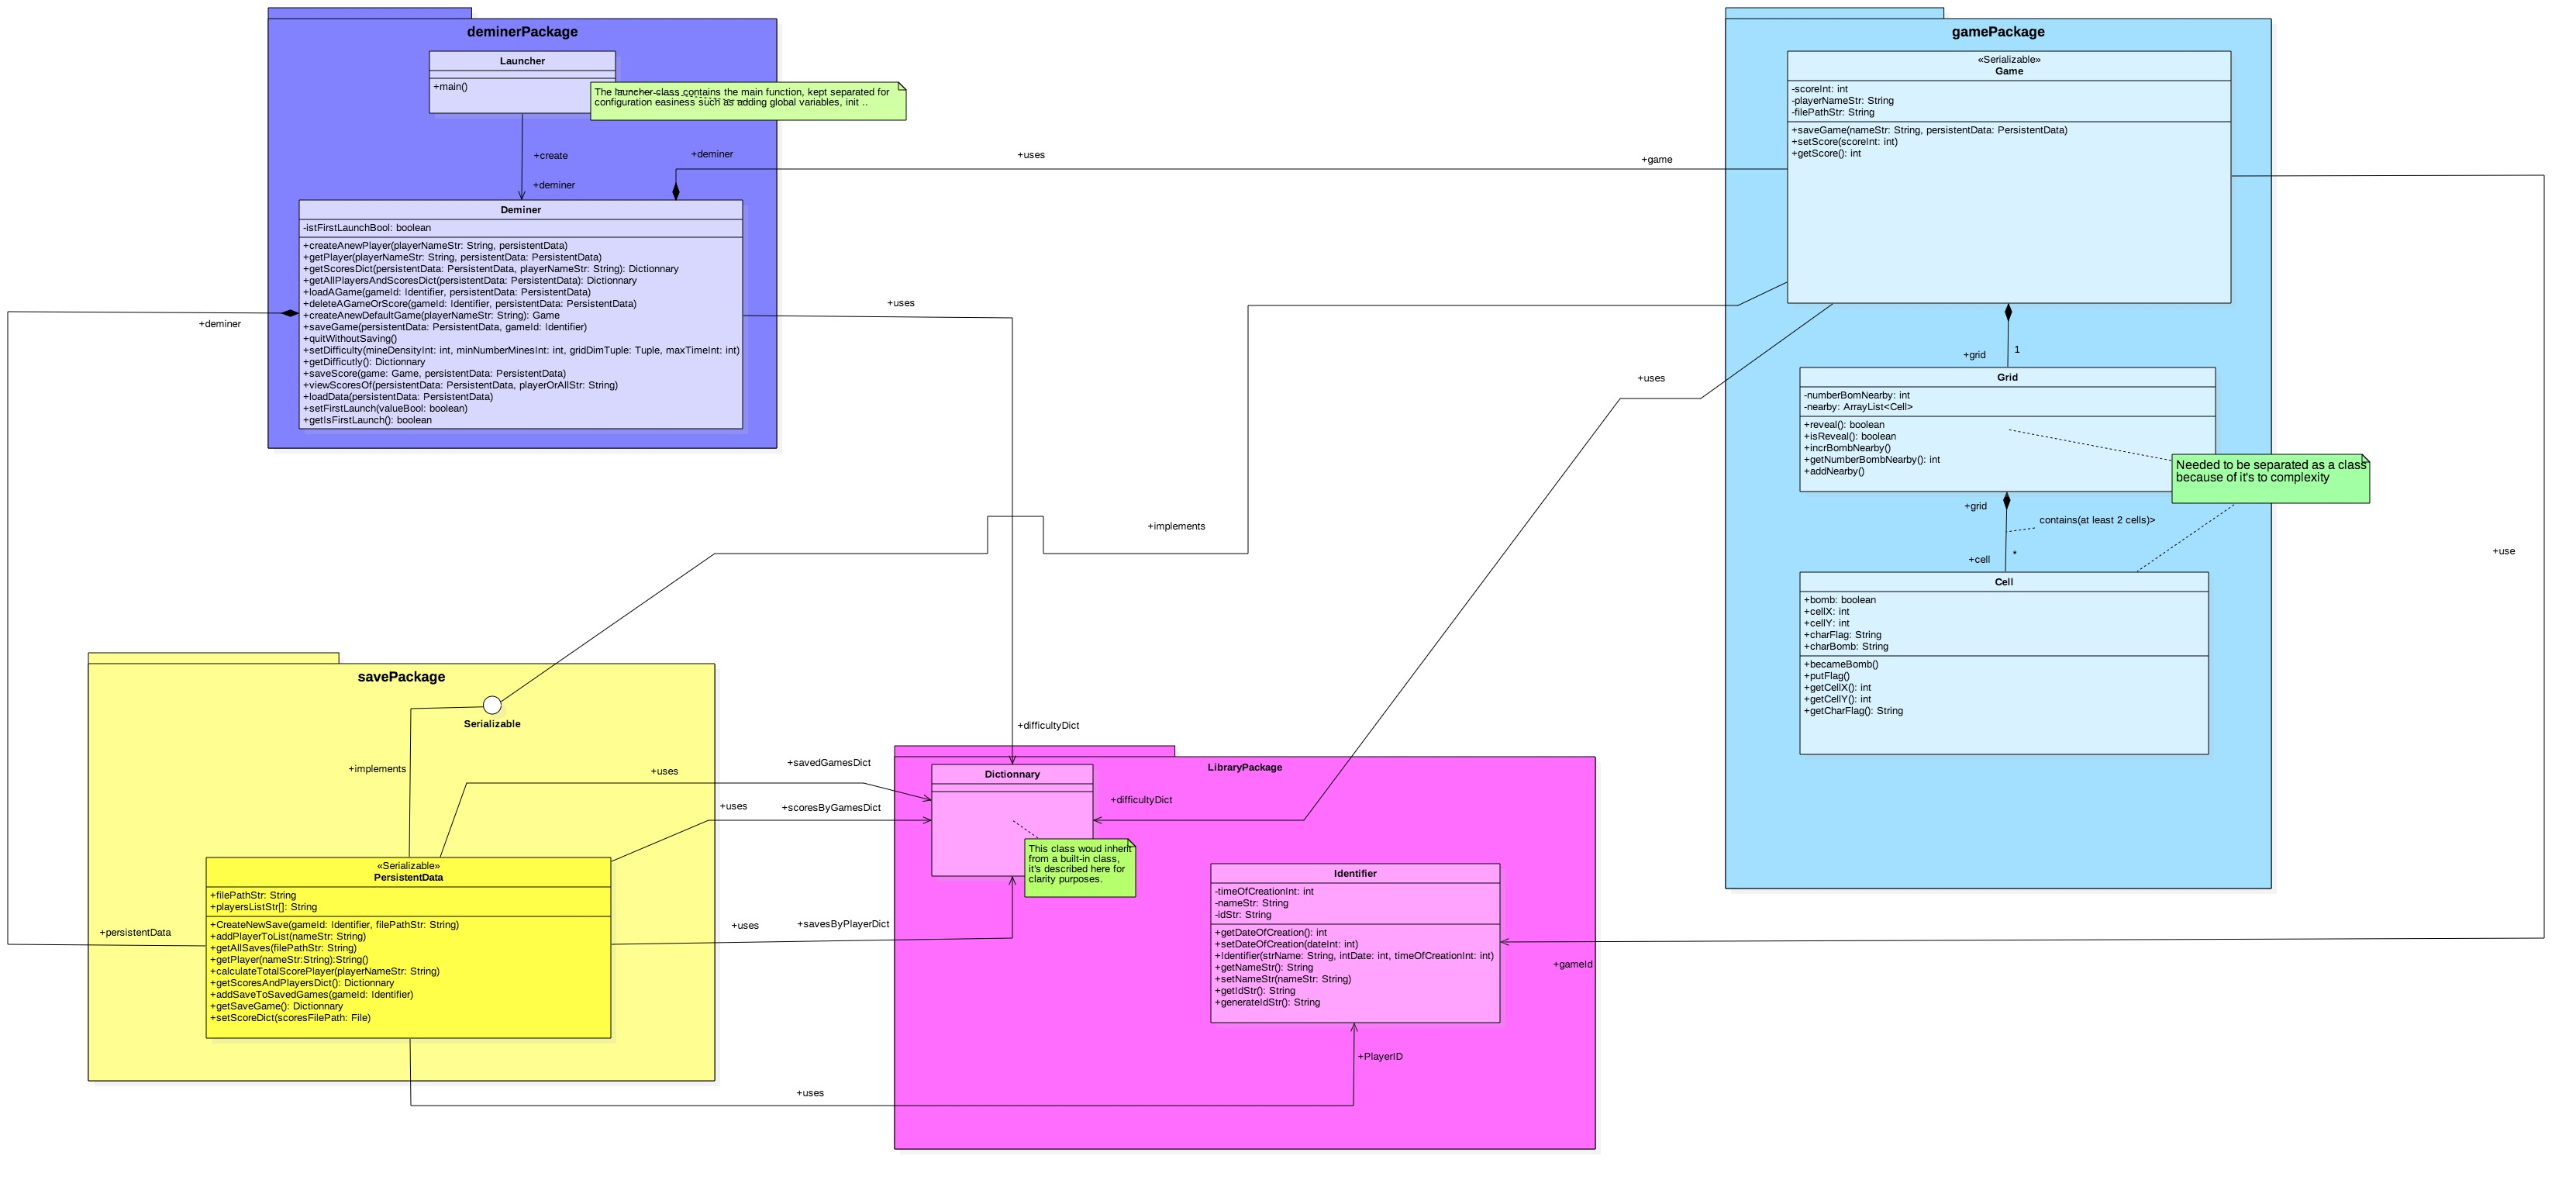
\includegraphics[scale=0.10]{Images/ClassDiagram.jpg}
	\end{block}
\end{frame}

%------------------------------------------------

\begin{frame}
	\begin{block}{Diagramme de cas d'utilisations}
		 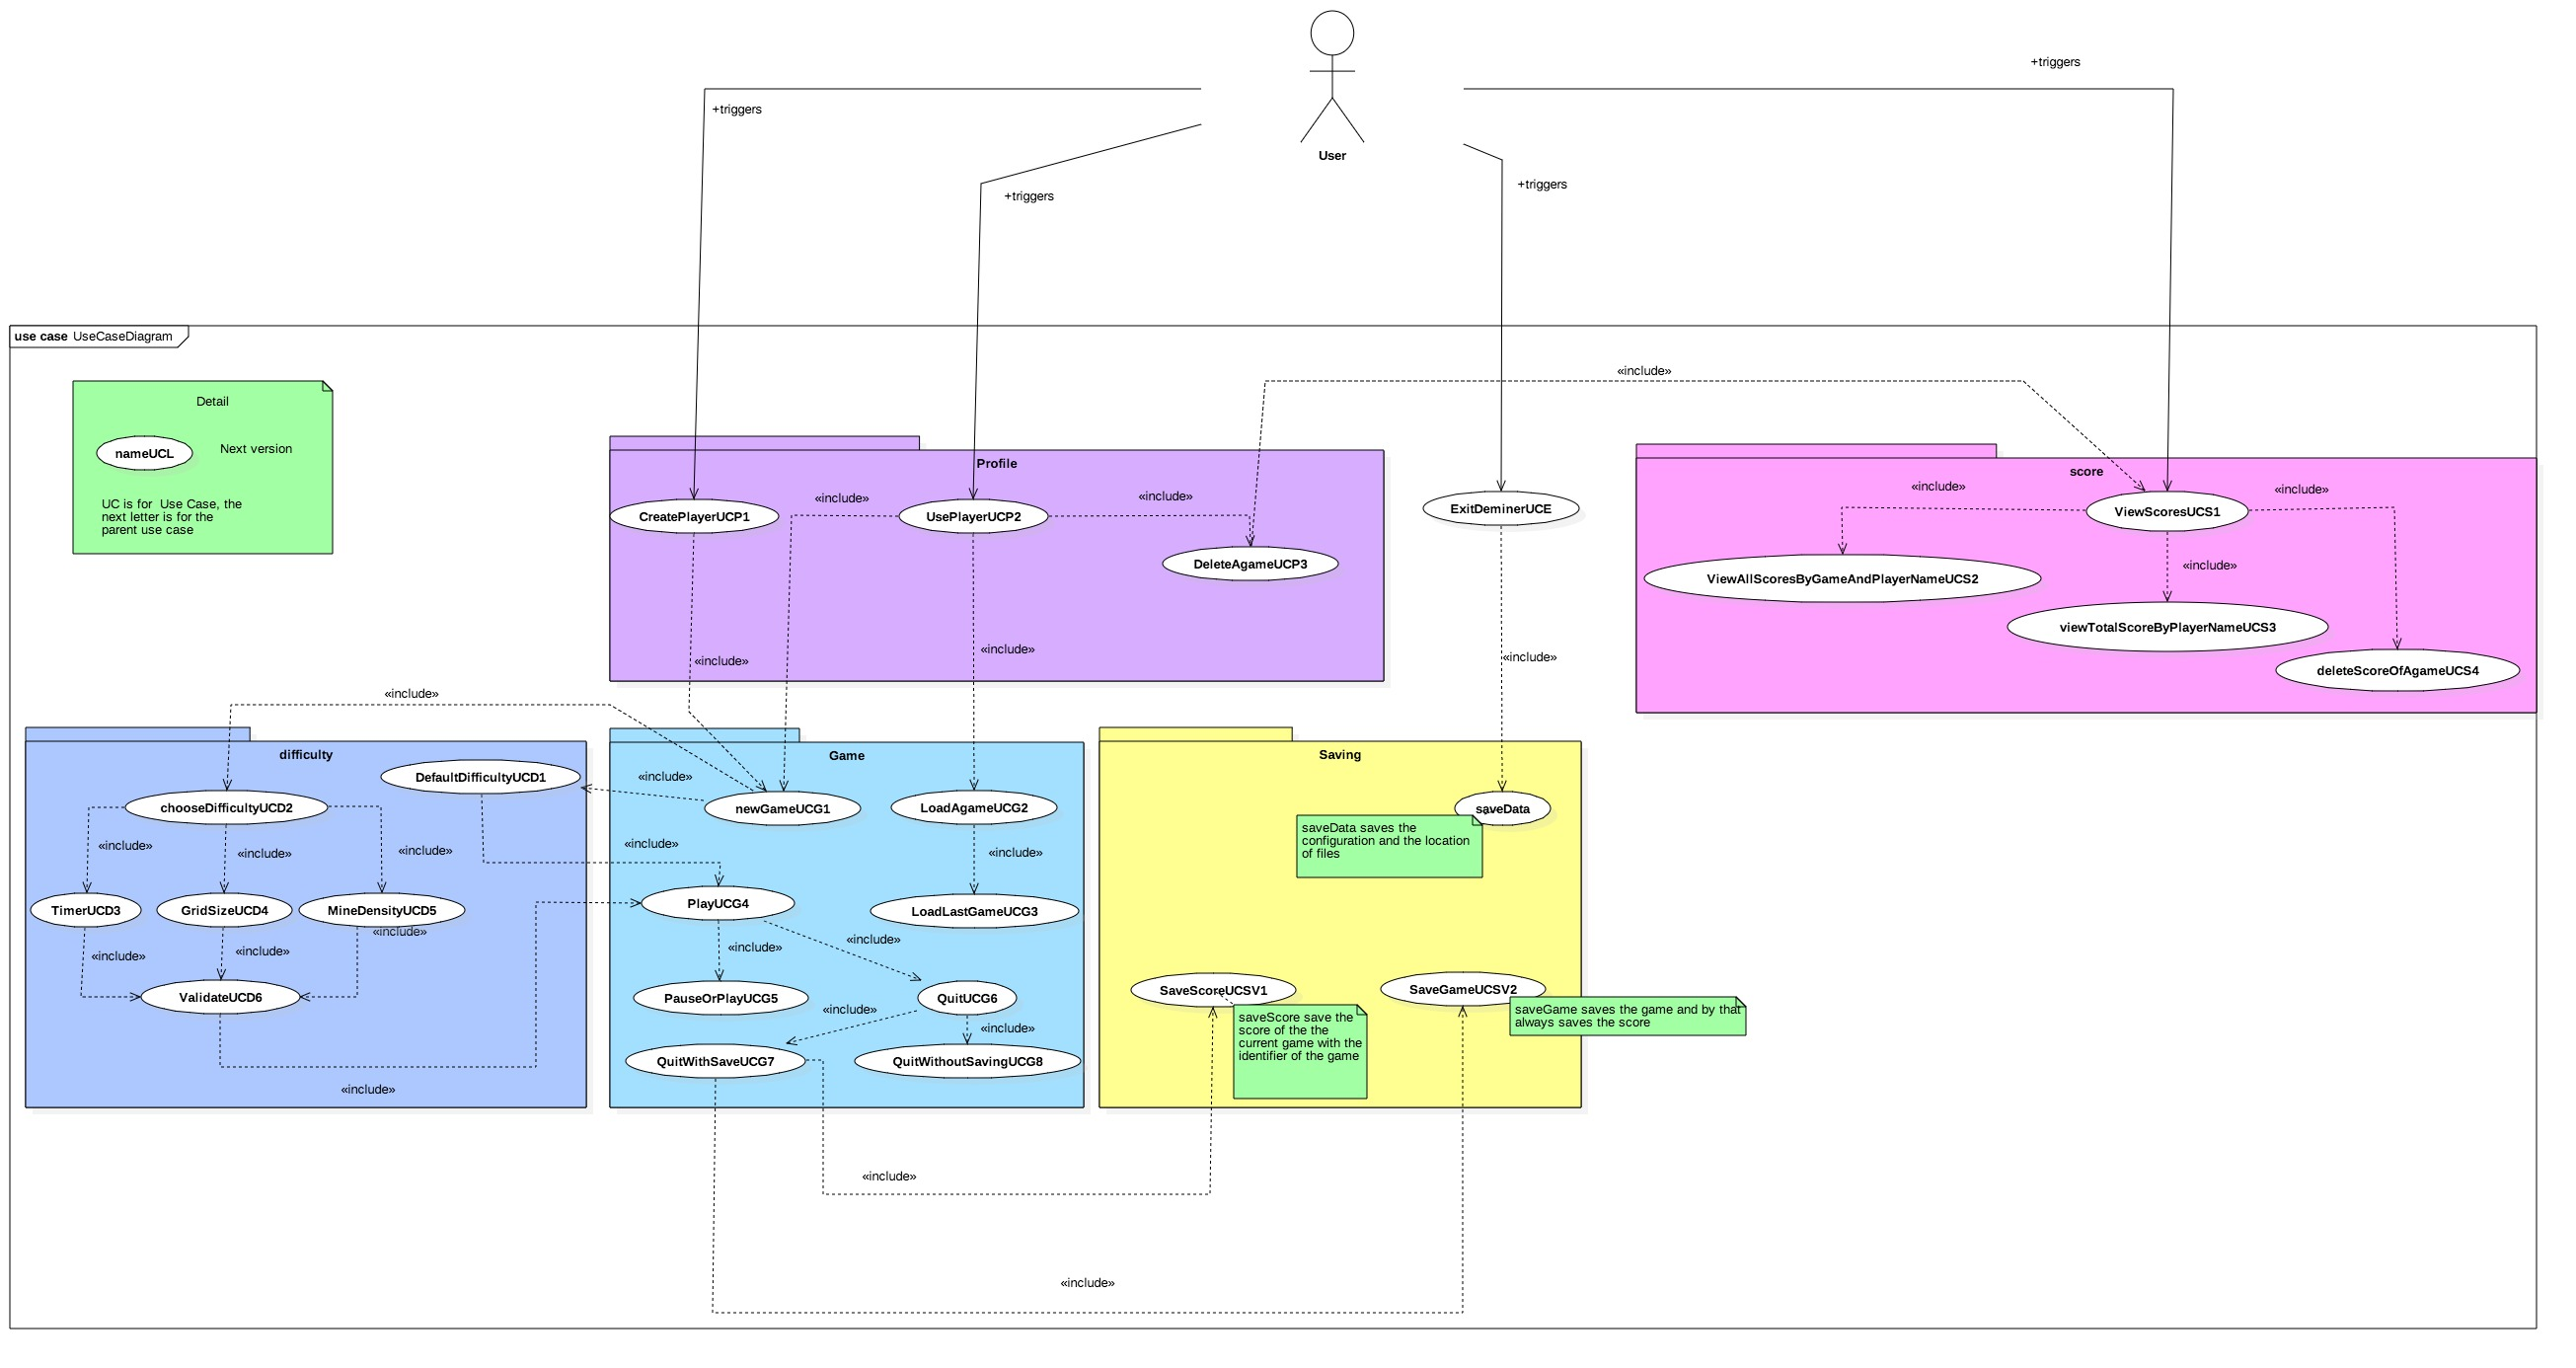
\includegraphics[scale=0.13]{Images/UseCaseDiagram.jpg}
	\end{block}
\end{frame}

%------------------------------------------------



%---------------------------------------------------------------------------------------------------------------------------------------------------------
\section{Android}
%---------------------------------------------------------------------------------------------------------------------------------------------------------

\begin{frame}
\begin{block}{Présentation}
   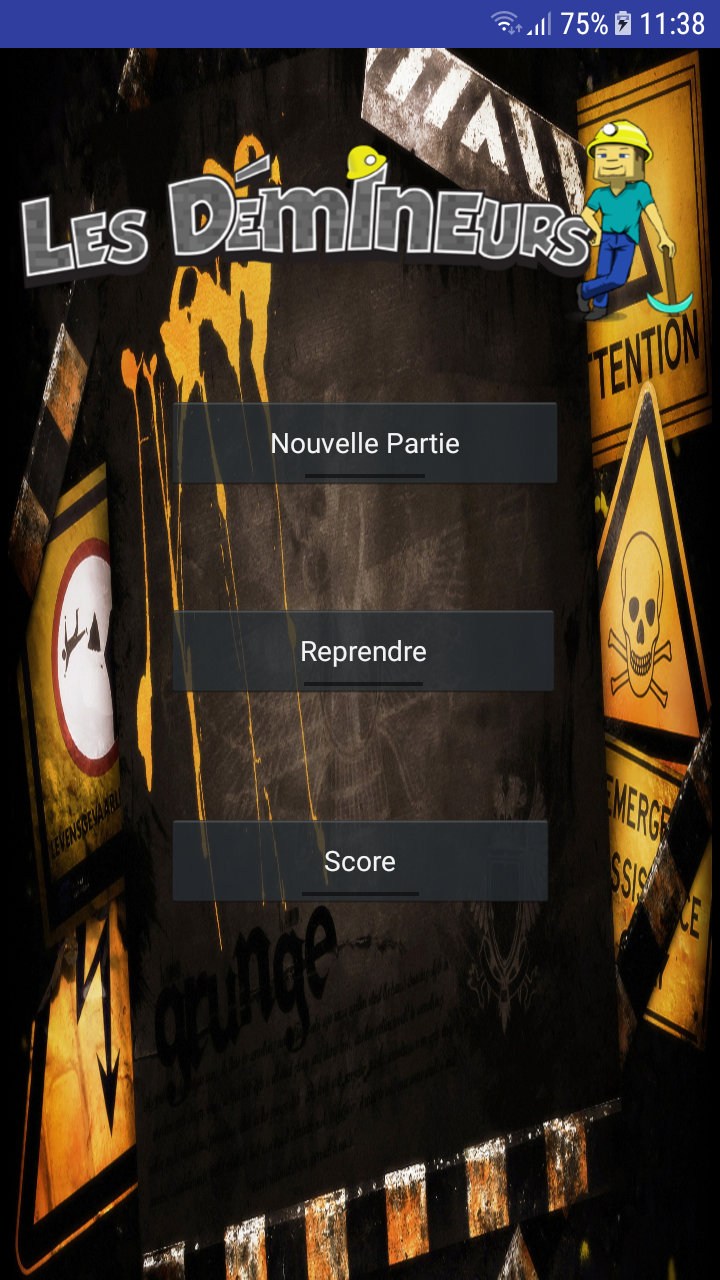
\includegraphics[scale=0.15]{Images/Main.png}
But: il vous faut déterminer l'emplacement de toutes les mines.
\end{block}

\end{frame}


%------------------------------------------------

\begin{frame}
\frametitle{Android}
\begin{block}{Présentation}
% Your image included here
    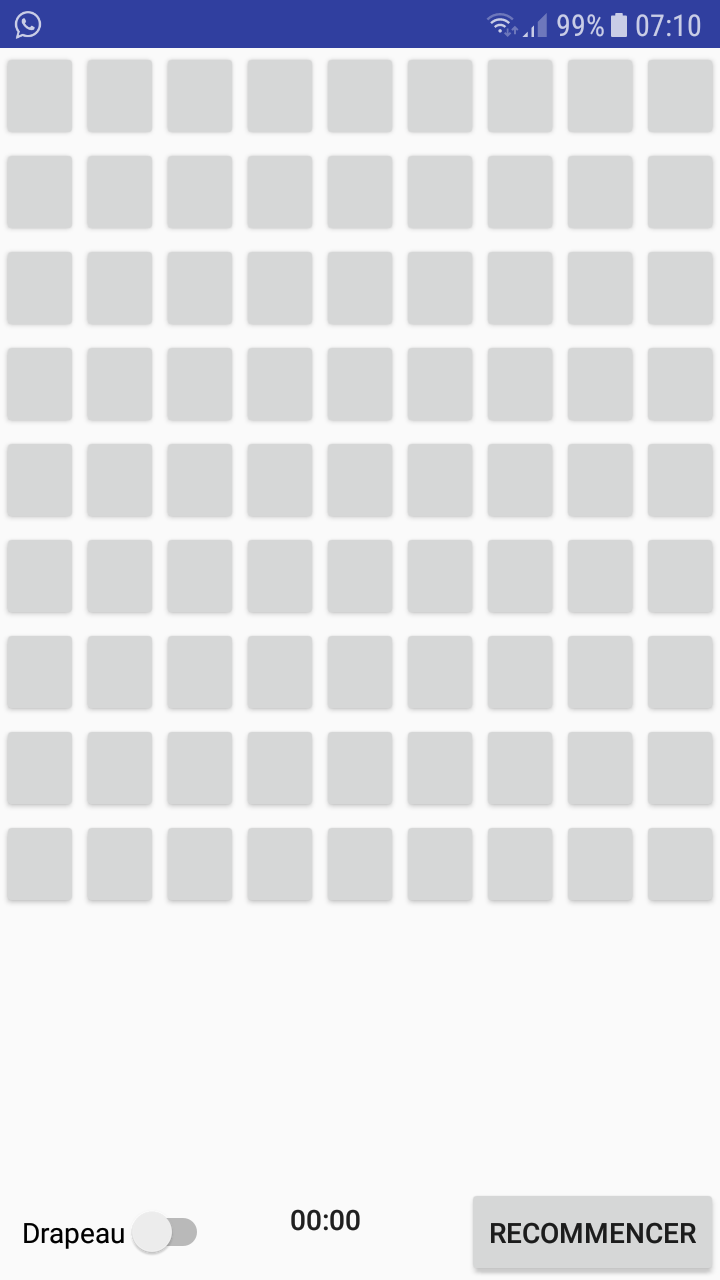
\includegraphics[scale=0.15]{Images/1.png}
    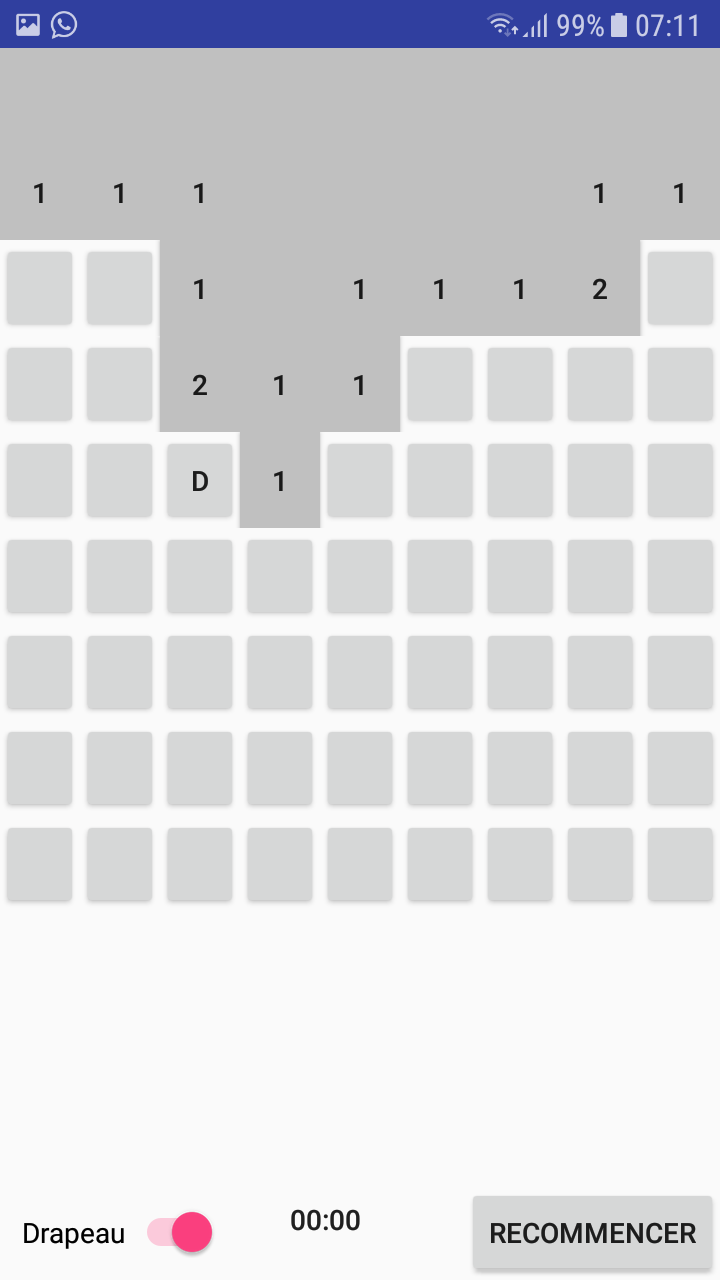
\includegraphics[scale=0.15]{Images/2.png}
    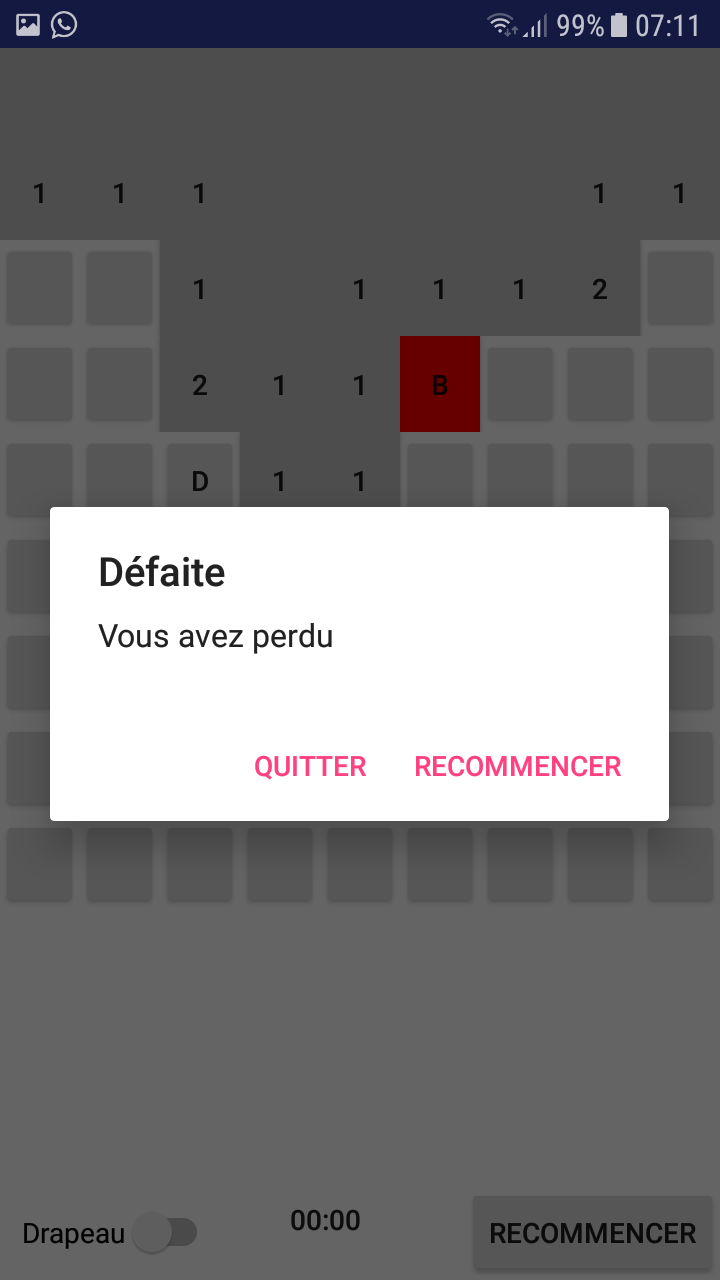
\includegraphics[scale=0.15]{Images/3.png}
\end{block}

\end{frame}

%------------------------------------------------
\begin{frame}
\begin{block}{Portion de code}
	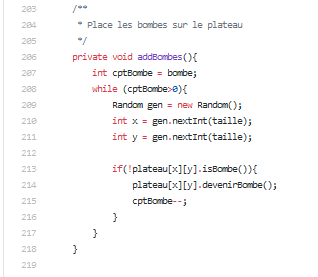
\includegraphics[scale=0.65]{Images/BombeRandom.png}
	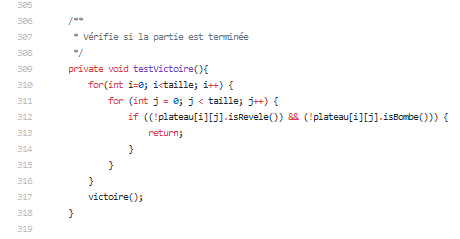
\includegraphics[scale=0.65]{Images/Victoire.png}
\end{block}
   
\end{frame}



%---------------------------------------------------------------------------------------------------------------------------------------------------------
\section{iOS}
%---------------------------------------------------------------------------------------------------------------------------------------------------------

\begin{frame}
\frametitle{iOS}
	\begin{block}{Storyboard et programmation  : MVC}
 		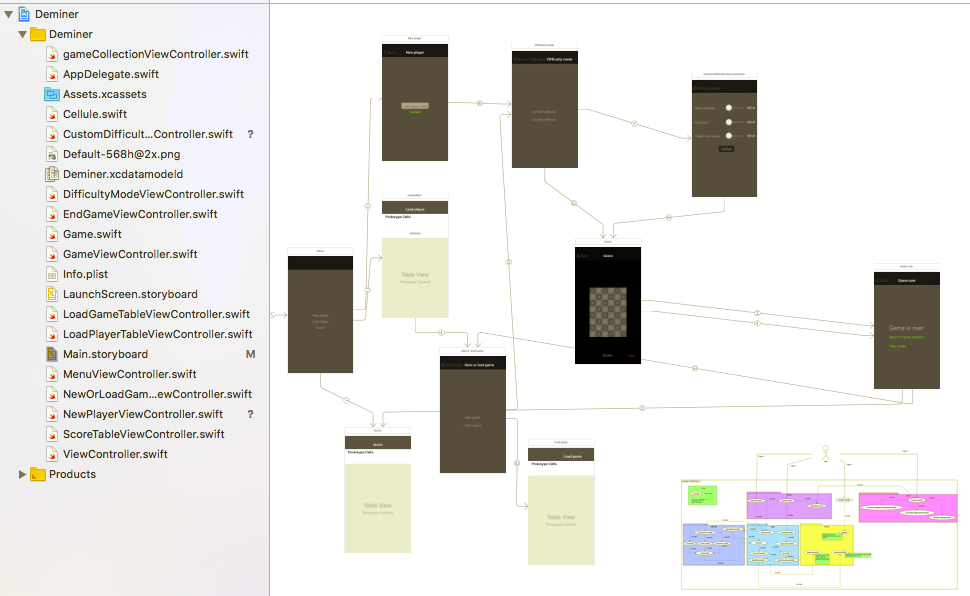
\includegraphics[scale=0.3]{Images/MVC.png}
	\end{block}
\end{frame}

\begin{frame}
\frametitle{iOS}
\begin{block}{Storyboard et programmation }
 		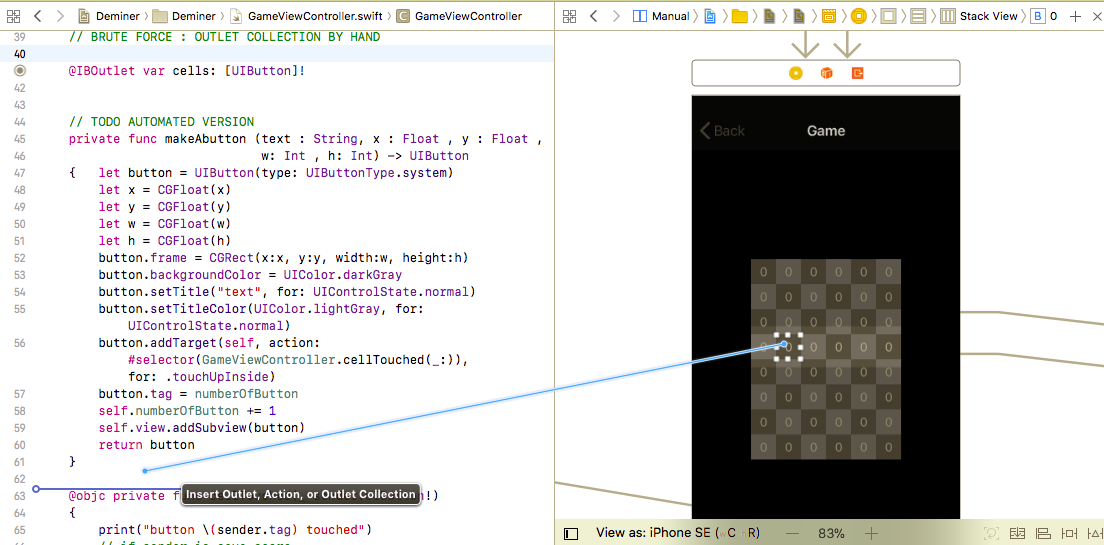
\includegraphics[scale=0.30]{Images/controlDrag.png}
	\end{block}

\end{frame}


\begin{frame}
	\frametitle{iOS}
	\begin{block}{Storyboard et programmation}
 		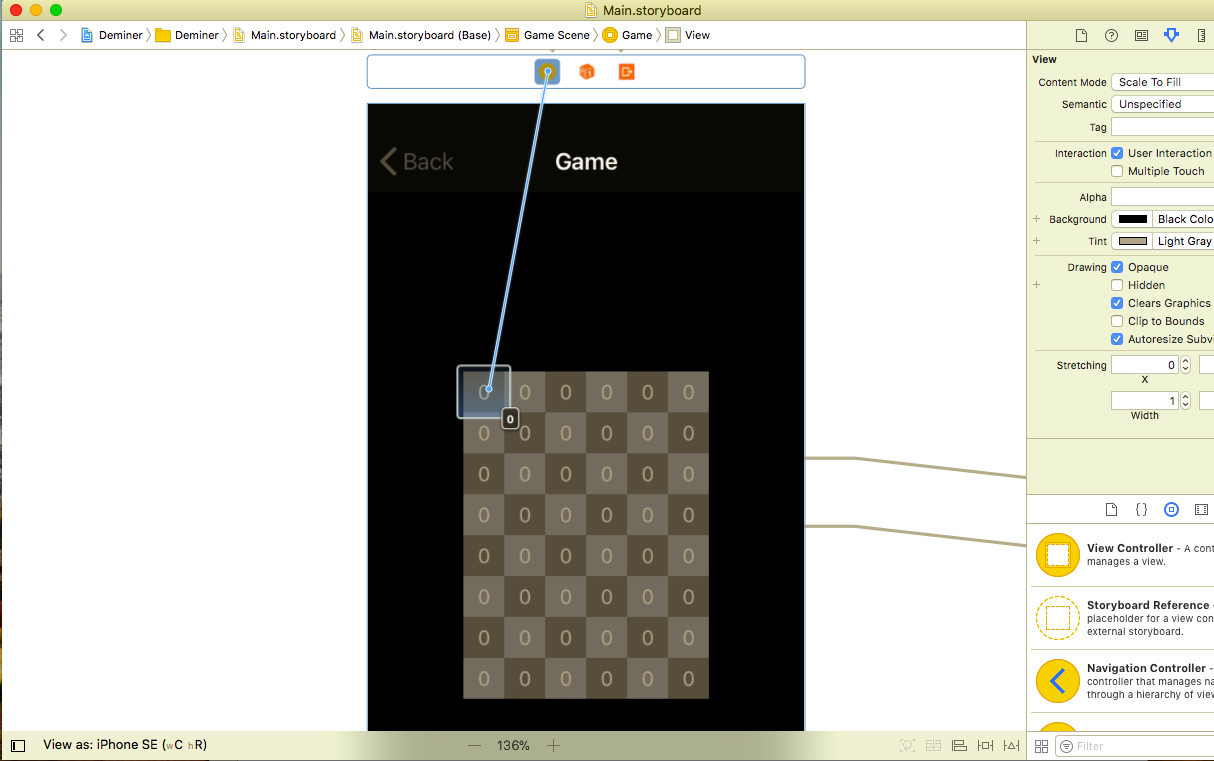
\includegraphics[scale=0.2]{Images/controlDragCollection.png}
	\end{block}
\end{frame}


\begin{frame}
\frametitle{iOS}
	\frametitle{iOS}
	\begin{block}{Persistance des données}
 		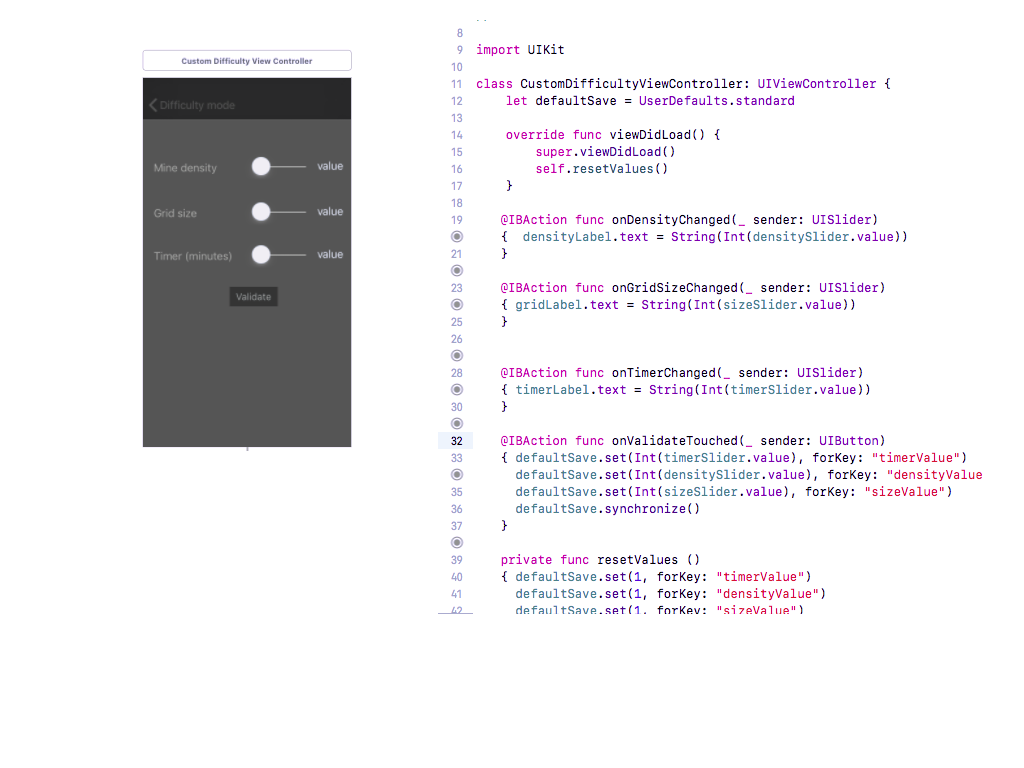
\includegraphics[scale=0.30]{Images/persistanceSliders.png}
	\end{block}
\end{frame}

%---------------------------------------------------------------------------------------------------------------------------------------------------------
\section{Conclusion}
%---------------------------------------------------------------------------------------------------------------------------------------------------------

\begin{frame}
\frametitle{Conclusion}
	\Huge{\centerline{Démonstration}}
\end{frame}

%------------------------------------------------

\begin{frame}
\Huge{\centerline{The End}}
\end{frame}

%----------------------------------------------------------------------------------------

\end{document} 